%% LyX 2.2.3 created this file.  For more info, see http://www.lyx.org/.
%% Do not edit unless you really know what you are doing.
\documentclass[12pt,english]{article}
\usepackage[osf]{mathpazo}
\renewcommand{\sfdefault}{lmss}
\renewcommand{\ttdefault}{lmtt}
\usepackage[T1]{fontenc}
\usepackage[latin9]{inputenc}
\usepackage[paperwidth=30cm,paperheight=35cm]{geometry}
\geometry{verbose,tmargin=2cm,bmargin=2cm}
\setlength{\parindent}{0bp}
\usepackage{amsmath}
\usepackage{amssymb}

\makeatletter
%%%%%%%%%%%%%%%%%%%%%%%%%%%%%% User specified LaTeX commands.
\usepackage{tikz}
\usetikzlibrary{matrix,arrows,decorations.pathmorphing}
\usetikzlibrary{shapes.geometric}
\usepackage{tikz-cd}
\usepackage{amsthm}
\usepackage{xparse,etoolbox}

\theoremstyle{plain}
\newtheorem{theorem}{Theorem}[section]
\newtheorem{lemma}[theorem]{Lemma}
\newtheorem{prop}{Proposition}[section]
\newtheorem*{cor}{Corollary}
\theoremstyle{definition}
\newtheorem{defn}{Definition}[section]
\newtheorem{ex}{Exercise} 
\newtheorem{example}{Example}[section]
\theoremstyle{remark}
\newtheorem*{rem}{Remark}
\newtheorem*{note}{Note}
\newtheorem{case}{Case}
\usepackage{graphicx}
\usepackage{amssymb}
\usepackage{tikz-cd}
\usetikzlibrary{calc,arrows,decorations.pathreplacing}
\tikzset{mydot/.style={circle,fill,inner sep=1.5pt},
commutative diagrams/.cd,
  arrow style=tikz,
  diagrams={>=latex},
}

\usepackage{babel}
\usepackage{hyperref}
\hypersetup{
    colorlinks,
    citecolor=blue,
    filecolor=blue,
    linkcolor=blue,
    urlcolor=blue
}
\usepackage{pgfplots}
\usetikzlibrary{decorations.markings}
\pgfplotsset{compat=1.9}


\newcommand{\blocktheorem}[1]{%
  \csletcs{old#1}{#1}% Store \begin
  \csletcs{endold#1}{end#1}% Store \end
  \RenewDocumentEnvironment{#1}{o}
    {\par\addvspace{1.5ex}
     \noindent\begin{minipage}{\textwidth}
     \IfNoValueTF{##1}
       {\csuse{old#1}}
       {\csuse{old#1}[##1]}}
    {\csuse{endold#1}
     \end{minipage}
     \par\addvspace{1.5ex}}
}

\raggedbottom

\blocktheorem{theorem}% Make theo into a block
\blocktheorem{defn}% Make defi into a block
\blocktheorem{lemma}% Make lem into a block
\blocktheorem{rem}% Make rem into a block
\blocktheorem{cor}% Make col into a block
\blocktheorem{prop}% Make prop into a block


\usepackage[bottom]{footmisc}

\makeatother

\usepackage{babel}
\begin{document}

\title{Homological Constructions over a Field of Characteristic $2$ }

\maketitle
~~~Throughout this section, let $K$ be a field of characteristic
$2$, $S$ denote the polynomial ring $K[x_{1},\dots,x_{n}]$, $I$
be a homogeneous ideal in $S$, and let $G$ be the reduced Gr�bner
basis for $I$ with respect to some fixed monomial ordering.

\section{Constructing the Chain Complexes $(S,d)$, $(S_{I},d)$, and $(I,\underline{d})$. }

\subsection{Construction of $(S,d)$}

~~~Let $d:S\to S$ be the graded $K$-linear map of degree $-1$
given by $d:=\sum_{j=1}^{n}\partial_{x_{j}}$. Since $K$ has characteristic
$2$, we have $d^{2}=0$. Indeed, it suffices to show that $d^{2}(m)=0$
for all monomials $m$ in $S$. So let $m=x_{1}^{\alpha_{1}}\cdots x_{n}^{\alpha_{n}}$
be a monomial in $S$. Then
\begin{align*}
d^{2}(m) & =\left(\sum_{k=1}^{n}\partial_{x_{k}}\right)^{2}\left(x_{1}^{\alpha_{1}}\cdots x_{n}^{\alpha_{n}}\right)\\
 & =\left(\sum_{k=1}^{n}\partial_{x_{k}}^{2}\right)\left(x_{1}^{\alpha_{1}}\cdots x_{n}^{\alpha_{n}}\right)\\
 & =\sum_{k=1}^{\infty}\alpha_{k}(\alpha_{k}-1)x_{1}^{\alpha_{k}-2}\\
 & =0.
\end{align*}

Thus the differential $d$ gives the graded $K$-module $S$ the structure
of a chain complex over $K$. 

\subsection{Construction of $(S_{I},d)$}

~~~Let $m=x_{1}^{\alpha_{1}}\cdots x_{n}^{\alpha_{n}}$ be a monomial
of degree $i$ in $S$. We denote 
\[
[m]_{o}=\{1\leq\lambda\leq n\mid\alpha_{\lambda}\text{ is odd}\}\qquad\text{and}\qquad[m]_{e}=\{1\leq\mu\leq n\mid\alpha_{\mu}\text{ is even}\}
\]
Using this notation, we can express the differential in another way:
\[
d(m)=\sum_{\lambda\in[m]_{o}}x_{\lambda}^{-1}m.
\]
This makes it clear that the differential $d$ maps $S_{I}$ into
$S_{I}$. Indeed, if $m$ is not in $\text{LT}(I)$, then every term
$x_{\lambda}^{-1}m$ of $d(m)$ is not in $\text{LT}(I)$ either.
Thus the differential $d$ gives the graded $K$-module $S_{I}$ the
structure of a chain complex over $K$. 

\subsection{Construction of $(S/I,\overline{d})$}

\begin{defn} We say $I$ is $d$-\textbf{stable }if $d$ maps $I$
into $I$. \end{defn}

~~~Suppose $I$ is $d$-stable. Then the differential $d:S\to S$
induces a graded linear map of degree $-1$, denoted $\overline{d}:S/I\to S/I$,
where 
\[
\overline{d}(\overline{f})=\overline{d(f)}\text{ for all }f\in S.
\]
Indeed, the map $\overline{d}$ is well-defined since $d$ is $I$-stable.
To see why, let $f+g$ and $f,$ where $g\in I$ and $f\in S$, be
two different representatives of a class in $S/I$, i.e. $\overline{f+g}=\overline{f}\in S/I$.
Then 
\begin{align*}
\overline{d}\left(\overline{f+g}\right) & =\overline{d(f+g)}\\
 & =\overline{d(f)+d(g)}\\
 & =\overline{d(f)}\\
 & =\overline{d}(\overline{f}).
\end{align*}

where $\overline{d(f)+d(g)}=\overline{d(f)}$ since $d(g)\in I$. 

~~~Moreover, the differential $\overline{d}$ gives $S/I$ the
structure of a differential graded $K$-algebra. Indeed, $\overline{d}$
is a graded linear map of degree $-1$ such that $\overline{d}^{2}=0$
and such that $\overline{d}$ satisfies Leibniz law. This is because
$\overline{d}$ inherits all of the properties from $d$. For instance,
to see that $\overline{d}$ satisfies Leibniz law, let $\overline{f}_{1}$
and $\overline{f}_{2}$ be in $S/I$. Then 
\begin{align*}
\overline{d}(\overline{f_{1}f_{2}}) & =\overline{d(f_{1}f_{2})}\\
 & =\overline{d(f_{1})f_{2}+f_{1}d(f_{2})}\\
 & =\overline{d(f_{1})f_{2}}+\overline{f_{1}d(f_{2})}\\
 & =\overline{d}(\overline{f_{1}})\overline{f_{2}}+\overline{f_{1}}\overline{d}(\overline{f_{2}}).
\end{align*}

Thus if $I$ is $d$-stable, then the differential $\overline{d}$
gives the graded $K$-algebra $S/I$ the structure of a differential
graded $K$-algebra. 

\subsection{Construction of $(I,\underline{d})$ }

~~~Our final construction involves the graded $K$-module $I$.
Let $\underline{d}:I\to I$ be the graded $K$-linear map of degree
$-1$ given by 
\[
\underline{d}(f):=d(f)+d(f)^{G}=\pi(d(f))
\]
for all $f\in I$. Then $\underline{d}^{2}=0$. Indeed, for all $f\in I$,
we have 
\begin{align*}
\underline{d}(\underline{d}(f)) & =\underline{d}(d(f)+d(f)^{G})\\
 & =d(d(f)+d(f)^{G})+d(d(f)+d(f)^{G})^{G}\\
 & =d(d(f)^{G})+d(d(f)^{G})^{G}\\
 & =d(d(f)^{G})+d(d(f)^{G})\\
 & =0,
\end{align*}
where $d(d(f)^{G})^{G}=d(d(f)^{G})$ since every term in $d(d(f)^{G})$
is not in $I$. Thus the differential $\underline{d}$ gives the graded
$K$-module $I$ the structure of a chain complex over $K$. 

\begin{rem}\label{remImodJ} Let $J$ be a homogeneous ideal in $S$
such that $I\supset J$. If $J$ is $\underline{d}$-stable, then
the differential $\underline{d}$ gives the graded $K$-module $I/J$
the structure of a chain complex over $K$, which we denote by $(I/J,\underline{d})$.
If $I$ and $J$ are both monomial ideals, then $J$ is always $\underline{d}$-stable.
\end{rem}

\section{Differential Graded $K$-Algebras }

~~~Since $d$ is defined in terms of partial derivatives, it is
clear that $d$ satisfies Leibniz law. Thus $(S,d)$ is more than
just a chain complex over $K$; it is a differential graded $K$-algebra.
Since $S_{I}$ is a graded $K$-algebra, it is natural wonder if $(S_{I},d)$
is also a differential graded $K$-algebra. A quick counterexample
shows that this is not necessarily the case:

\begin{example}\label{example} Consider $S=K[x]$ and $I=\langle x^{5}\rangle$.
Then
\begin{align*}
d(x\cdot x^{4}) & =d((x^{5})^{G})\\
 & =d(0)\\
 & =0,
\end{align*}
but 
\begin{align*}
d(x)\cdot x^{4}+x\cdot d(x^{4}) & =1\cdot x^{4}+x\cdot0\\
 & =(x^{4})^{G}+0^{G}\\
 & =x^{4},
\end{align*}
so $d(x\cdot x^{5})\neq d(x)\cdot x^{4}+x\cdot d(x^{4})$. \end{example}

\subsection{When $(S_{I},d)$ Has the Structure of a Differential Graded $K$-Algebra }

~~~The next theorem tells us precisely when $(S_{I},d)$ is a differential
graded $K$-algebra. 

\begin{theorem}\label{theoremdgalgebrasi} $(S_{I},d)$ is a differential
graded $K$-algebra if and only if $d(g)=0$ for all $g\in G$. \end{theorem}

\begin{proof} Assume that $d(g)=0$ for all $g\in G$. We first prove
that $d(f^{G})=d(f)^{G}$ for all $f\in S$. Let $f\in S$. From the
division algorithm, we have $f=g_{1}q_{1}+\cdots+g_{r}q_{r}+f^{G}$
for some $q_{1},\dots,q_{r}\in S$. Thus 
\begin{align*}
d(f) & =d(g_{1}q_{1}+\cdots+g_{r}q_{r}+f^{G})\\
 & =d(g_{1}q_{1})+\cdots+d(g_{r}q_{r})+d(f^{G})\\
 & =g_{1}d(q_{1})+\cdots+g_{r}d(q_{r})+d(f^{G}).
\end{align*}
Since $g_{1}d(h_{1})+\cdots+g_{r}d(h_{r})\in I$ and no term of $d(f^{G})$
is divisible by any element of $\text{LT}(I)$, it follows from uniqueness
of normal forms that $d(f^{G})=d(f)^{G}$. 

~~~Now we show that this implies that $(S_{I},d)$ is a differential
graded $K$-algebra. Let $f_{1},f_{2}\in S_{I}$. Then 
\begin{align*}
d(f_{1}\cdot f_{2}) & =d((f_{1}f_{2})^{G})\\
 & =(d(f_{1}f_{2}))^{G}\\
 & =(d(f_{1})f_{2}+f_{1}d(f_{2}))^{G}\\
 & =(d(f_{1})f_{2})^{G}+(f_{1}d(f_{2}))^{G}\\
 & =d(f_{1})\cdot f_{2}+f_{1}\cdot d(f_{2}).
\end{align*}

Therefore $(S_{I},d)$ is a differential graded $K$-algebra. 

~~Now we prove the converse. Assume $(S_{I},d)$ is a differential
graded $K$-algebra. Let $g\in G$ and let $m$ be the lead term of
$g$. We may assume $g$ is not a constant (otherwise we'd clearly
have $d(g)=0$). Thus, there exists some $x_{\lambda}$ such that
$x_{\lambda}$ divides $m$. Then on the one hand, we have
\begin{align*}
d(x_{\lambda}\cdot x_{\lambda}^{-1}m) & =d(m^{G})\\
 & =d(g+m)\\
 & =d(g)+d(m),
\end{align*}
since $m^{G}=g+m$. On the other hand, we have 
\begin{align*}
d(x_{\lambda})\cdot x_{\lambda}^{-1}m+x_{\lambda}\cdot d(x_{\lambda}^{-1}m) & =(x_{\lambda}^{-1}m)^{G}+(x_{\lambda}d(x_{\lambda}^{-1}m))^{G}\\
 & =x_{\lambda}^{-1}m+(x_{\lambda}d(x_{\lambda}^{-1}m))^{G}\\
 & =x_{\lambda}^{-1}m+(x_{\lambda}(x_{\lambda}^{-2}m+x_{\lambda}^{-1}d(m)))^{G}\\
 & =x_{\lambda}^{-1}m+(x_{\lambda}^{-1}m+d(m))^{G}\\
 & =x_{\lambda}^{-1}m+(x_{\lambda}^{-1}m)^{G}+d(m)^{G}\\
 & =x_{\lambda}^{-1}m+x_{\lambda}^{-1}m+d(m)^{G}\\
 & =d(m),
\end{align*}

since $(x_{\lambda}^{-1}m)^{G}=x_{\lambda}^{-1}m$ and $d(m)^{G}=d(m)$
(every term of $d(m)$ does not lie in $\langle\text{LT}(G)\rangle$).
Since $(S_{I},d)$ is a differential graded $K$-algebra, we must
have $d(g)=0$. This establishes this theorem. \end{proof}

\begin{rem}\label{rem} We should note that the identity $x_{\lambda}d(x_{\lambda}^{-1}m)=x_{\lambda}(x_{\lambda}^{-2}m+x_{\lambda}^{-1}d(m))=x_{\lambda}^{-1}m+d(m)$
follows since $d$ satisfies Leibniz law not just in $S$, but also
in $S[x_{1}^{-1},\dots,x_{n}^{-1}]$. Again, this is because $d$
is defined in terms of partial derivatives. \end{rem}

\begin{example}\label{example} Going back to Example~(\ref{examplediffalgSI}),
where $S=K[x,y]$, $I=\langle xy^{2}+y^{3},x^{3}+x^{2}y\rangle$,
and $G=\{xy^{2}+y^{3},x^{3}+x^{2}y\}$. We have $d(xy^{2}+y^{3})=d(x^{3}+x^{2}y)=0$.
Therefore Proposition~(\ref{propdgalgebrasi}) implies $(S_{I},d)$
is a differential graded $K$-algebra. \end{example}

~~~Now we want to show that $(S_{I},d)$ is a differential graded
$K$-algebra if and only if $(S/I,\overline{d})$ is a differential
graded $K$-algebra, and moreover, they are isomorphic to each other. 

\begin{lemma}\label{lemmadg} Let $I$ be a homogeneous ideal in the
polynomial ring $S$, and let $G=\{g_{1},g_{2},\dots,g_{r}\}$ be
the reduced Gr�bner basis for $I$. Then $d(g)=d(g)^{G}$ for all
$g\in G$. \end{lemma} 

\begin{proof} Let $g\in G$. If $d(g)=0$, then clearly we have $d(g)=d(g)^{G}$,
so assume $d(g)\neq0$. We need to prove that $d(g)=d(g)^{G}$. This
is equivalent to saying that no term of $d(g)$ belongs to $\langle\text{LT}(G)\rangle:=\langle\text{LT}(g_{1}),\text{LT}(g_{2}),\dots,\text{LT}(g_{r})\rangle$,
since $G$ is a Gr�bner basis. Every term in of $d(g)$ has the form
$x_{\lambda}^{-1}m$ where $m$ is some term of $g$. It is easy to
see that this term cannot belong to $\text{\ensuremath{\langle}LT}(G)\rangle$.
Indeed, if $x_{\lambda}^{-1}m\in\langle\text{LT}(G)\rangle$, then
$m\in\langle\text{LT}(g_{2}),\dots,\text{LT}(g_{r})\rangle$, and
this contradicts the fact that $G$ is a \emph{reduced }Gr�bner basis.
\end{proof}

\begin{prop}\label{propcriteriondstable} $I$ is $d$-stable if and
only if $d(g)\in I$ for all $g\in G$. \end{prop}

\begin{proof} One direction is trivial, so let's prove the other
direction. Suppose $d(g)\in I$ for all $g\in G$ and let $f\in I$.
Since $G$ generates $I$, we can write $f=\sum_{\lambda=1}^{r}q_{\lambda}g_{\lambda}$
for some $q_{1},\dots,q_{r}\in S$. Thus, by Leibniz law, we have
\begin{align*}
d(f) & =d\left(\sum_{\lambda=1}^{r}q_{\lambda}g_{\lambda}\right)\\
 & =\sum_{\lambda=1}^{r}d(q_{\lambda}g_{\lambda})\\
 & =\sum_{\lambda=1}^{r}(d(q_{\lambda})g_{\lambda}+q_{\lambda}d(g_{\lambda}))\in I.
\end{align*}
Thus, $I$ is $d$-stable. \end{proof} 

~~~Combining Lemma~(\ref{lemmadg}) and Proposition~(\ref{propcriteriondstable}),
we find that that $d(g)=0$ for all $g\in G$ if and only if $d(g)\in I$
for all $g\in G$ if and only if $I$ is $d$-stable. Combining this
with Theorem~(\ref{theoremdgalgebrasi}), we find that $(S_{I},d)$
is a differential graded $K$-algebra if and only if $(S/I,\overline{d})$
is a differential graded $K$-algebra. Now we will show that they
are in fact isomorphic to each other. 

\begin{theorem}\label{theoremdifferentialgradedalgebraI} Suppose
$I$ is $d$-stable. Then $(S_{I},d)$ is isomorphic to $(S/I,\overline{d})$
as differential graded $K$-algebras. \end{theorem}

\begin{proof} Recall that $S/I$ is isomorphic to $S_{I}$ as graded
$K$-algebras, where the isomorphism is given by mapping $\overline{f}\in S/I$
to $f^{G}\in S_{I}$. It remains to show that this isomorphism respects
the differential graded algebra structure. In particular, we need
to show that $d(f^{G})=d(f)^{G}$ for all $f\in S$. This was already
proven in Theorem~(\ref{theoremdgalgebrasi}). \end{proof}

\subsection{More Differential Graded $K$-algebras}

\begin{prop}\label{prop} Suppose $I$ is $d$-stable and let $g$
be a homogeneous polynomial such that $d(g)=0$. Then $(S_{\langle I,g\rangle},d)$
and $(S_{I:g},d)$ are differential graded $K$-algebras. \end{prop}

\begin{proof} We just need to show that $\langle I,g\rangle$ and
$I:g$ are both $d$-stable. Since $d(g)=0$, it follows that $\langle I,g\rangle$
is $d$-stable. To prove that $I:g$ is $d$-stable, let $f\in I:g$.
Then since $fg\in I$, $d(g)=0$, and $I$ is $d$-stable, it follows
that 
\[
d(f)g=d(f)g+fd(g)=d(fg)\in I
\]
Therefore $d(f)\in I:g$, which implies that $I:g$ is $d$-stable.
\end{proof}

\begin{example}\label{example} Consider $S=K[x,y,z]$, $g=x^{2}y+x^{2}z$,
and $I=\langle f_{1},f_{2},f_{3}\rangle$ where
\begin{align*}
f_{1} & =xy+xz+yz\\
f_{2} & =x^{4}y+x^{5}\\
f_{3} & =y^{3}+y^{2}z
\end{align*}
Then $d(f_{1})=d(f_{2})=d(f_{3})=0$ implies that $(S_{I},d)$ is
a differential graded $K$-algebra. The reduced Gr�bner basis for
$I$ with respect to graded lexicographical ordering is $G=\{g_{1},g_{2},g_{3},g_{4},g_{5},g_{6}\}$,
where 
\begin{align*}
g_{1} & =xy+xz+yz\\
g_{2} & =y^{3}+y^{2}z\\
g_{3} & =y^{2}z^{2}\\
g_{4} & =xz^{4}+yz^{4}\\
g_{5} & =x^{5}+x^{4}z+x^{3}z^{2}+x^{2}z^{3}\\
g_{6} & =x^{4}z^{2}
\end{align*}

Since $d(g)=0$, we know that $(S_{\langle I,g\rangle},d)$ and $(S_{I:g},d)$
are also differential graded $K$-algebras. The reduced Gr�bner basis
for $I:g$ with respect to graded lexicographical ordering is $G''=\{g_{1}'',g_{2}'',g_{3}''\}$,
where 
\begin{align*}
g_{1}'' & =y+z\\
g_{2}'' & =z^{2}\\
g_{3}'' & =x^{3}+x^{2}z
\end{align*}
and the reduced Gr�bner basis for $\langle I,g\rangle$ with respect
to graded lexicographical ordering is $G'=\{g_{1}',g_{2}',g_{3}',g_{4}',g_{5}'\}$,
where 
\begin{align*}
g_{1}' & =xy+xz+yz\\
g_{2}' & =y^{3}+y^{2}z\\
g_{3}' & =xz^{2}+yz^{2}\\
g_{4}' & =y^{2}z^{2}\\
g_{5}' & =x^{5}+x^{4}z+x^{3}z^{2}+x^{2}z^{3}
\end{align*}

\end{example}

\section{Homology Calculations}

\subsection{$H(S/I,\overline{d})\protect\cong0$ }

\begin{prop}\label{propSisfree} Suppose $I$ is $d$-stable. Then
$H(S_{I})=0$. \end{prop}

\begin{proof} Let $f$ be a homogeneous polynomial in $S_{I}$ such
that $d(f)=0$. Then for any $x_{\lambda}\in(S_{I})_{1}$, we have
\[
d(x_{\lambda}f)=d(x_{\lambda})f+x_{\lambda}d(f)=f.
\]
Therefore $\text{Ker}(d)=\text{Im}(d)$, hence $H(S_{I})=0$. \end{proof}

\begin{rem}\label{remSIisfreeforspecialG} Taking $I=0$ shows that
$H(S)=0$. \end{rem}

\subsection{$H_{i}(I)\protect\cong H_{i-1}(S_{I})$ }

\begin{prop}\label{proplongexact} The differential $d$ induces isomorphisms
$H_{i}(I)\cong H_{i-1}(S_{I})$ for all $i>0$. \end{prop}

\begin{proof} First we show that $\underline{d}\pi=\pi d$. For all
$f\in S$, we have
\begin{align*}
\underline{d}(\pi(f)) & =\underline{d}(f+f^{G})\\
 & =d(f+f^{G})+d(f+f^{G})^{G}\\
 & =d(f)+d(f^{G})+d(f)^{G}+d(f^{G})^{G}\\
 & =d(f)+d(f^{G})+d(f)^{G}+d(f^{G})\\
 & =d(f)+d(f)^{G}\\
 & =\pi(d(f)),
\end{align*}

where $d(f^{G})^{G}=d(f^{G})$ because no term in $d(f^{G})$ lies
in $\text{LT}(I)$. 

~~~Therefore we have a short exact sequence of chain complexes
over $K$:

\begin{center}\begin{tikzcd} 0 \arrow[r] & (S_I ,d )  \arrow[r] & (S,d) \arrow[r, " \pi "] &  (I,\underline{d} ) \arrow[r] &  0.  \end{tikzcd}\end{center}

From this, we obtain a long exact sequence in homology, which gives
for each $i>0$, the following short exact sequences:

\begin{center}\begin{tikzcd} 0 = H_i (S) \arrow[r] & H_i (I) \arrow[r, "d"] &  H_{i-1}(S_I ) \arrow[r] & H_{i-1}(S ) = 0.  \end{tikzcd}\end{center}

where $d$ is obtained from the connecting map. In more detail, $d$
maps the element $[f]\in H_{i}(I)$ to the element $[d(f)]\in H_{i-1}(S_{I})$.
\end{proof}

\subsection{Decomposing $H_{i}(S_{I})$ }

~~~Let $g$ be a homogeneous polynomial of degree $j$ and let
$G'$ be the reduced Gr�bner basis for $\langle I,g\rangle$ with
respect to our fixed monomial ordering. In Commutative Algebra, we
learn about the following short exact sequence of graded $S$-modules\begin{center}\begin{tikzcd}[row sep=5] 0 \arrow[r] & (S/(I:g))(-j) \arrow[r, "g"] & S/I \arrow[r] & S/\langle I \text{,} g \rangle \arrow[r] & 0 

\\

& \overline{f} \arrow[r,mapsto,shorten >=0.5cm,shorten <=0.5cm] & \overline{fg}
\end{tikzcd}\end{center}

We want to use this short exact sequence to our advantage. First,
using the isomorphisms $S_{I:g}\cong S/(I:g)$, $S_{I}\cong S/I$,
and $S_{\langle I,g\rangle}\cong S/\langle I,g\rangle$, we get, for
each $i$, a short exact sequence of $K$-vector spaces

\begin{center}\begin{tikzcd}[row sep=5] 0 \arrow[r] & (S_{I:g} )_{j-i} \arrow[r, "\cdot g"] & (S_I )_i \arrow[r, "-^{G'} "] & ( S _{\langle I \text{,} g \rangle })_i \arrow[r] & 0 

\\

& f \arrow[r,mapsto,shorten >=0.5cm,shorten <=0.5cm] & (fg)^G

\\

&& f \arrow[r,mapsto,shorten >=0.5cm,shorten <=0.5cm] & f^{G' }
\end{tikzcd}\end{center}



or in other words, a short exact sequence of graded $K$-vector spaces 

\begin{center}\begin{tikzcd}[row sep=5] 0 \arrow[r] & (S_{I:g})(-j)  \arrow[r, "\cdot g"] & S_I  \arrow[r,"-^{G'} "] & S _{\langle I \text{,} g \rangle } \arrow[r] & 0

\end{tikzcd}\end{center}

We want to know under what conditions this becomes a short exact sequence
of chain complexes over $K$, that is, when does the following diagram
commute?

\begin{center}\begin{tikzcd} & \vdots \arrow[d] & \vdots \arrow[d] & \vdots \arrow[d]

\\

0 \arrow[r] & (S_{I:g} )_{j-i} \arrow[d,"d",swap] \arrow[r, "\cdot g"] & (S_I )_i \arrow[d,"d",swap] \arrow[r, "-^{G'} "] & ( S _{\langle I \text{,} g \rangle })_i \arrow[r] \arrow[d,"d"] & 0 

\\

0 \arrow[r] & (S_{I:g} )_{j-i-1} \arrow[d] \arrow[r, "\cdot g"] & (S_I )_{i-1} \arrow[d] \arrow[r, "-^{G'} "] & ( S _{\langle I \text{,} g \rangle })_{i-1} \arrow[d] \arrow[r] & 0 

\\

& \vdots  & \vdots  & \vdots

\end{tikzcd}\end{center}

After some thought, we find that the conditions which need to be satisfied
are the following:
\begin{equation}
(gd(m))^{G}=d((gm)^{G})\text{ for all monomials }m\text{ which are not in }\text{LT}(I:g)\label{eq:condition1}
\end{equation}
\begin{equation}
d(m)^{G'}=d(m^{G'})\text{ for all monomials }m\text{ which are not in }\text{LT}(I)\label{eq:condition2}
\end{equation}

For the moment, let's assume that these conditions are satisfied so
that we have a short exact sequence of chain complexes. Then by the
usual argument, the short exact sequence of chain complexes gives
rise to a long exact sequence in homology:

\begin{center}\begin{tikzcd}[row sep=40]  && \cdots \arrow[r] \arrow[d, phantom, ""{coordinate, name=Z'}] & H_{i+1} (S _{\langle I \text{,} g \rangle }) \arrow[dll, " \lambda ", swap, rounded corners, to path={ -- ([xshift=2ex]\tikztostart.east) |- (Z') [near end]\tikztonodes -| ([xshift=-2ex]\tikztotarget.west) -- (\tikztotarget)}] 



\\  & H_{i-j} (S_{I:g} ) \arrow[r, "\cdot g"] & H_{i} (S_I ) \arrow[r, "-^{G'} "] \arrow[d, phantom, ""{coordinate, name=Z}] & H_{i} (S _{\langle I \text{,} g \rangle }) \arrow[dll, " \lambda ", swap, rounded corners, to path={ -- ([xshift=2ex]\tikztostart.east) |- (Z) [near end]\tikztonodes -| ([xshift=-2ex]\tikztotarget.west) -- (\tikztotarget)}] 

\\ & H_{i-j-1} (S_{I:g} ) \arrow[r, "\cdot g "] & H_{i-1} (S_I ) \arrow[r, "-^{G'} "] & \cdots 

\end{tikzcd}\end{center}

It's easy to see that the connecting maps $\lambda$ all induce the
zero map. So in fact, we get for each $i$, the short exact sequence
of $K$-vector spaces:

\begin{center}\begin{tikzcd}[row sep=40] 0 \arrow[r]  & H_{i-j} (S_{I:g} ) \arrow[r, "\cdot g"] & H_{i} (S_I ) \arrow[r,"-^{G'} "] & H_{i} (S _{\langle I \text{,} g \rangle }) \arrow[r] & 0,  

\end{tikzcd}\end{center}

and since the inclusion map $S_{\langle I,g\rangle}\hookrightarrow S_{I}$
splits the map $-^{G'}$, we obtain the following isomorphism
\begin{equation}
H_{i-j}(S_{I:g})\oplus H_{i}(S_{\langle I,g\rangle})\cong H_{i}(S_{I})\label{eq:homologydirectsum}
\end{equation}

where we map the representative $(f_{1},f_{2})$ in $H_{i-j}(S_{I:g})\oplus H_{i}(S_{\langle I,g\rangle})$
to the representative $gf_{1}+f_{2}$ in $H_{i}(S_{I})$.

\subsubsection{Decomposing $H_{i}(S_{I})$ in a Special Case and an Example}

~~~We will now discuss a special case of when the conditions in
Theorem~(\ref{theoremdecomposition}) are satisfied. Consider the
case where $I$ is a monomial ideal and $g$ is a monomial of degree
$j$ which is not in $I$. Then condition (\ref{eq:condition1}) is
satisfied since if $m$ is not in $I:g$, then $gm$ is not in $I$,
and so $(gm)^{G}=gm$ which implies $(gd(m))^{G}=gd(m)$. 

~~~For condition (\ref{eq:condition2}) first assume that $m$
is not in $\langle I,g\rangle$. Then then $m^{G'}=m$, which implies
$d(m)^{G'}=d(m)=d(m^{G'})$. Thus condition (\ref{eq:condition2})
is satisfied in this case. Now assume that $m=g$. Then $m^{G'}=0$,
which implies $d(m^{G'})=0$. Thus, we must have $d(g)=0$ in order
for condition (\ref{eq:condition2}) to be satisfied in this case.
So assume $d(g)=0$ and consider the final case where $m=m_{1}g$.
Since $d(g)=0$, we obtain $d(m)^{G'}=(d(m_{1})g)^{G'}=0$, and thus
(\ref{eq:condition2}) is satisfied in this case as well. 

~~~In the next example, we show how we can apply Theorem~(\ref{theoremdecomposition})
recursively. In what follows, we frequently use the notation $I,g$
to mean $\langle I,g\rangle$ and $I:g$ to mean $I:\langle g\rangle$.
For example, $I,g_{1}:g_{2}=\langle I,g_{1}\rangle:\langle g_{2}\rangle$,
and $I:g_{1},g_{2}=\langle(I:g_{1}),\langle g_{2}\rangle\rangle$,
and so on. We also note that $I:g_{1}:g_{2}=I:g_{1}g_{2}$. 

\begin{example}\label{examplerecursivehomology} Consider $S=K[x,y,z]$
and $I=\langle x^{3}y,yz^{3}\rangle$. Then $d(x^{2})=d(z^{2})=0$,
and so 
\begin{align*}
H_{i}(S_{I}) & =x^{2}H_{i-2}(S_{I:x^{2}})\oplus H_{i}(S_{I,x^{2}})\\
 & =x^{2}(z^{2}H_{i-4}(S_{I:x^{2}z^{2}})\oplus H_{i-2}(S_{I:x^{2},z^{2}}))\oplus z^{2}H_{i-2}(S_{I,x^{2}:z^{2}})\oplus H_{i}(S_{I,x^{2},z^{2}})\\
 & =x^{2}z^{2}H_{i-4}(S_{I:x^{2}z^{2}})\oplus x^{2}H_{i-2}(S_{I:x^{2},z^{2}})\oplus z^{2}H_{i-2}(S_{I,x^{2}:z^{2}})\oplus H_{i}(S_{I,x^{2},z^{2}})
\end{align*}

We calculate
\begin{align*}
I:x^{2}z^{2} & =\langle xy,yz\rangle\\
I,x^{2}:z^{2} & =\langle x^{2},yz\rangle\\
I:x^{2},z^{2} & =\langle xy,z^{2}\rangle\\
I,x^{2},z^{2} & =\langle x^{2},z^{2}\rangle
\end{align*}

The only part which has nontrivial homology is $S_{I:x^{2}z^{2}}$.
Thus, $H_{5}(S_{I})=[d(x^{3}yz^{2})]K$ and $H_{i}(S_{I})=0\text{ for }$all
$i\neq5$. \end{example}

\section{Constructing the Cochain Complexes $(S,\delta)$, $(S_{I},\delta)$,
and $(I,\delta)$ }

~~~For a $K$-vector space $V$, let $V^{\star}:=\text{Hom}_{K}(V,K)$.
We refer to $V^{\star}$ as the \textbf{dual }of $V$. If $\varphi:V\to W$
is a $K$-linear map from the vector space $V$ to the vector space
$W$, then we denote the $K$-linear map $\text{Hom}_{K}(\varphi,K):\text{Hom}_{K}(W,K)\to\text{Hom}_{K}(V,K)$
simply as $\varphi^{\star}$ and call it the \textbf{dual }of $\varphi$. 

\subsection{Construction of $(S,\delta)$ and $(I,\delta)$ }

~~~The duals of $S_{I}$, $S$, and $I$ are all graded $K$-modules,
where the homogeneous components are simply the duals of $(S_{I})_{i}$,
$S_{i}$, and $I_{i}$ respectively. In fact, $S_{I}$, $S/I$, $S$,
and $I$ are all isomorphic as graded $K$-modules to their duals:
To get an isomorphism from $S_{i}$ to $S_{i}^{\star}$, we map the
monomial $x^{\alpha}\in S_{i}$ to the element $\underline{x}^{\alpha}\in S_{i}^{\star}$,
where $\underline{x}^{\alpha}$ is defined on the monomial $x^{\beta}\in S_{i}$
as 
\[
\underline{x}^{\alpha}(x^{\beta})=\begin{cases}
0 & \text{if }\alpha\neq\beta\\
1 & \text{if }\alpha=\beta
\end{cases}
\]
and is extended linearly everywhere else. The isomorphisms $(S_{I})_{i}^{\star}\cong(S_{I})_{i}$
and $I_{i}^{\star}\cong I_{i}$ are induced from this isomorphism. 

~~~We can describe $d^{\star}$ as follows: Let $m=x_{1}^{\alpha_{1}}\cdots x_{n}^{\alpha_{n}}$
be a monomial of degree $i-1$ in $S$. Then
\[
d^{\star}(\underline{m})=\sum_{\mu\in[m]_{e}}\underline{x^{\mu}m}.
\]
Using the isomorphism from $S$ to $S^{\star}$ described above, we
pull $d^{\star}$ back to a map on $S$ and we denote this map as
$\delta$ and call it the \textbf{codifferential}. Thus, for each
monomial $m\in S$, we have 
\begin{equation}
\delta(m)=\sum_{\mu\in[m]_{e}}x_{\mu}m.\label{eq:deltadescription}
\end{equation}
It is clear that $\delta$ is a graded endomorphism of $S$ of degree
$1$ such that $\delta^{2}=0$, and thus gives $S$ the structure
of a cochain complex over $K$. 

\begin{rem} Note that $(S,\delta)$ is not a differential graded
$K$-algebra with respect to the usual multiplication maps. For instance,
consider $S=K[x,y]$. Then $\delta(xy)=0$ but $\delta(x)y+x\delta(y)=x^{2}y+xy^{2}$.
Later on we will introduce a product, called \textbf{cup product},
which will give $(S,\delta)$ the structure of a differential graded
$K$-algebra with respect to this product. \end{rem}

\subsection{Construction of $(I,\delta)$}

Using the description of $\delta$ in (\ref{eq:deltadescription})
and the fact that $I$ is an ideal, we see that $\delta$ restricts
to a map $\delta:I\to I$, which is also a graded endomorphism of
$S$ of degree $1$ such that $\delta^{2}=0$, and thus gives $I$
the structure of a cochain complex over $K$. 

\subsubsection{Kronecker Pairing}

~~~When we identify monomials $\underline{x}^{\alpha}$ in $S^{\star}$
with monomials $x^{\alpha}$ in $S_{i}$, we are forgetting the way
monomials in $S_{i}^{\star}$ act on monomials in $S_{i}$. To make
up for this, we introduce a symmetric bilinear form $\langle\cdot,\cdot\rangle$
on $S_{i}$ called the \textbf{Kronecker pairing}: For monomials $x^{\alpha}$
and $x^{\beta}$ in $S_{i}$, we set
\[
\langle x^{\alpha},x^{\beta}\rangle=\underline{x}^{\alpha}(x^{\beta})=\begin{cases}
0 & \text{if }\alpha\neq\beta\\
1 & \text{if }\alpha=\beta
\end{cases}.
\]

Then we extend this linearily to $\langle\cdot,\cdot\rangle:S_{i}\times S_{i}\to K$.
From the way we constructed $\delta$, we have for all $f_{1},f_{2}\in S_{i}$,
we have $\langle\delta(f_{1}),f_{2}\rangle=\langle f_{1},d(f_{2})\rangle$. 

\subsection{Construction of $(S_{I},\delta)$ }

~~~Let $\underline{\delta}:S_{I}\to S_{I}$ be the graded $K$-linear
map of degree $1$ given by 
\[
\underline{\delta}(f):=\delta(f)^{G}
\]
for all $f\in S_{I}$. The map $\underline{\delta}$ gives the graded
$K$-module $S_{I}$ the structure of a cochain complex over $K$. 

\subsection{Cup and Cap Product}

~~~We introduce some notation. Let $m=x_{1}^{\alpha_{1}}\cdots x_{n}^{\alpha_{n}}$
be a monomial in $S$. If $\alpha_{\lambda}>0$, then we say $x_{\lambda}$
is in the \textbf{support }of $m$. We denote by $\text{supp}(m)$
to be the set of all $x_{\lambda}$ in the support of $m$. We will
assume that $x_{1}>x_{2}>\cdots>x_{n}$. We say $x_{\lambda}$ is
the \textbf{last nonzero coordinate }of $m$ if $x_{\lambda}$ is
the smallest element in $\text{supp}(m)$. We say $x_{\lambda}$ is
the \textbf{first nonzero coordinate }of $m$ if $x_{\lambda}$ is
the largest element in $\text{supp}(m)$. 

\subsubsection{Cup Product}

\begin{defn}\label{defn} Let $m_{1}$ and $m_{2}$ be monomials $S_{i}$
and $S_{j}$ respectively. The \textbf{cup product }of $m_{1}$ and
$m_{2}$ is 

\[
m_{1}\smile m_{2}=\begin{cases}
\frac{m_{1}m_{2}}{x_{\lambda}} & \text{if }x_{\lambda}\text{ is the last nonzero coordinate of }m_{1}\text{ and the first nonzero coordinate of }m_{2}\\
0 & \text{otherwise}
\end{cases}
\]

This extends to a linear map $\smile:S_{i}\times S_{j}\to S_{i+j-1}$
which we call the cup product. \end{defn}

\begin{example}\label{example} Let $S=K[x,y,z]$. Then 
\begin{align*}
(x^{2}y+xy^{2})\smile(x^{5}+y^{4}z) & =x^{2}y\smile x^{5}+xy^{2}\smile x^{5}+x^{2}y\smile y^{4}z+xy^{2}\smile y^{4}z\\
 & =x^{2}y\smile y^{4}z+xy^{2}\smile y^{4}z\\
 & =x^{2}y^{4}z+xy^{5}z.
\end{align*}

\end{example}

\begin{prop}\label{prop} Let $m_{1}$ and $m_{2}$ be two monomials
in $S$. Then
\begin{equation}
\delta(m_{1}\smile m_{2})=\delta(m_{1})\smile m_{2}+m_{1}\smile\delta(m_{2}).\label{eq:leibnizlawcodifferential}
\end{equation}
\end{prop}

\begin{proof} Let $x_{\lambda_{1}}$ be the last nonzero coordinate
of $m_{1}$ and let $x_{\lambda_{2}}$ be the first nonzero coordinate
of $m_{2}$. First assume that $x_{\lambda_{1}}>x_{\lambda_{2}}$.
Then $m_{1}\smile m_{2}=0$, and this implies $\delta(m_{1}\smile m_{2})=0$.
Also, the last nonzero coordinate of every monomial in $\delta(m_{1})$
will be greater than or equal to $x_{\lambda_{1}}$ which is strictly
greater than $x_{\lambda_{2}}$. Therefore $\delta(m_{1})\smile m_{2}=0$.
Similarly, the first nonzero in $\delta(m_{2})$ will be smaller than
or equal to $x_{\lambda_{2}}$ which is strictly smaller than $x_{\lambda_{1}}$.
Therefore $m_{1}\smile\delta(m_{2})=0$. So we trivially have (\ref{eq:leibnizlawcodifferential})
in this case. 

~~~Now we assume $x_{\lambda_{2}}>x_{\lambda_{1}}$. Then $m_{1}\smile m_{2}=0$,
and this implies $\delta(m_{1}\smile m_{2})=0$. Also, since $x_{\lambda_{1}}\in[m_{2}]_{e}$
and $x_{\lambda_{2}}\in[m_{1}]_{e}$, we will have $\delta(m_{1})\smile m_{2}=m_{1}m_{2}$
and $m_{1}\smile\delta(m_{2})=m_{1}m_{2}$. Adding everything together,
we get 
\[
\delta(m_{1}\smile m_{2})=0=\delta(m_{1})\smile m_{2}+m_{1}\smile\delta(m_{2}).
\]
~~~Finally, assume $x_{\lambda_{1}}=x_{\lambda_{2}}$. Let's denote
this common variable as $x_{\mu}$. On the one hand, we have 
\[
\delta(m_{1}\smile m_{2})=\delta\left(\frac{m_{1}m_{2}}{x_{\mu}}\right)=\sum_{\substack{x_{\lambda}\in[m_{1}]_{e}\\
x_{\lambda}\leq x_{\mu}
}
}\frac{x_{\lambda}m_{1}m_{2}}{x_{\mu}}+\sum_{\substack{x_{\lambda}\in[m_{2}]_{e}\\
x_{\lambda}\geq x_{\mu}
}
}\frac{x_{\lambda}m_{1}m_{2}}{x_{\mu}}
\]
On the other hand, we have 
\[
\delta(m_{1})\smile m_{2}=\sum_{\substack{x_{\lambda}\in[m_{1}]_{e}\\
x_{\lambda}\leq x_{\mu}
}
}\frac{x_{\lambda}m_{1}m_{2}}{x_{\mu}}\qquad\text{and}\qquad m_{1}\smile\delta(m_{2})=\sum_{\substack{x_{\lambda}\in[m_{2}]_{e}\\
x_{\lambda}\geq x_{\mu}
}
}\frac{x_{\lambda}m_{1}m_{2}}{x_{\mu}}.
\]
Combining these together gives the desired result. \end{proof}

\subsubsection{Cap Product}

\begin{defn}\label{defn} Let $m_{1}$ and $m_{2}$ be monomials $S_{i}$
and $S_{j}$ respectively. The \textbf{cap product }of $m_{1}$ and
$m_{2}$ is
\[
m_{1}\frown m_{2}=\begin{cases}
x_{\lambda}\frac{m_{2}}{m_{1}} & \text{if }m_{1}\mid m_{2},\text{ }x_{\lambda}\text{ is the last nonzero coordinate of }m_{1}\text{, and }x_{\lambda}\text{ is the first nonzero coordinate of }\frac{x_{\lambda}m_{2}}{m_{1}}.\\
0 & \text{otherwise}
\end{cases}
\]
The cap product extends linearly to a map $\frown:S_{i}\times S_{j}\to S_{i-j+1}$.
\end{defn}

\section{Topological Interpretation of $H(S_{I})$}

~~~In this section, we give a topological interpretation of $H(S_{I})$.
Since $H(S_{\text{LT}(I)})\cong H(S_{I})$, we only need to consider
the case where $I$ is a monomial ideal. Moreover, by using Theorem~(\ref{theoremdecomposition}),
we can specialize further to the case that $I$ is a squarefree monomial
ideal before tackling the more general case. Thus we will assume that
$I$ is a squarefree monomial ideal in this section. Our goal is to
show that $H(S_{I})$ is isomorphic to the simplicial homology of
a simplicial complex which is associated with $I$. 

\subsection{Reinterpreting Simplicial Complexes}

~~~We want to reinterpret the theory simplicial complexes using
the language of monomials. There is a bijection between the set of
subsets of $\{x_{1},\dots,x_{n}\}$ and the set of squarefree monomials
in the variables $x_{1},\dots,x_{n}$. Indeed, if $m$ is a squarefree
monomial, then the corresponding subset of $\{x_{1},\dots,x_{n}\}$
is $\text{supp}(m)$. Moreover, if $m$ and $m'$ are squarefree monomials,
then $m$ divides $m'$ if and only if $\text{supp}(m)\subseteq\text{supp}(m')$.
Here's how we think of the squarefree monomials in $x,y,z$ sit on
the $2$-simplex:

\begin{center}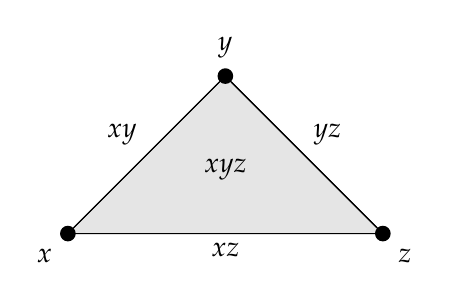
\begin{tikzpicture}

\draw[fill=gray!20] (0,0) -- (2,2) -- (4,0)-- (0,0);

\node[circle, fill=black, inner sep=2pt, label=below left:$x $] (a) at (0,0) {};
\node[circle, fill=black, inner sep=2pt, label=above :$y $] (b) at (2,2) {};
\node[circle, fill=black, inner sep=2pt, label=below right:$z $] (c) at (4,0) {};


\draw[] (a) -- (b) node [midway, above left] {$ xy $};
\draw[] (b) -- (c) node [midway, above right] {$ yz $};
\draw[] (c) -- (a) node [midway, below ] {$ xz $};

\node[label=below:$xyz$] (f) at (2,1.2) {};




\end{tikzpicture} \end{center}

\subsection{Stanley-Reisner Rings}

\subsubsection{Stanley-Reisner Ring}

~~~Let $\Delta$ be a simplicial complex on $\{x_{1},\dots,x_{n}\}$.
We denote by $I_{\Delta}$ to be the ideal of nonfaces of $\Delta$,
that is, $I_{\Delta}$ is generated by the squarefree monomials $m$
in $S$ which are not in $\Delta$. We define the \textbf{Stanley-Reisner
ring }$K[\Delta]$ of the simplicial complex $\Delta$ to be the $K$-algebra
$K[\Delta]:=S/I_{\Delta}$. We will also denote by $I_{\Delta}^{\text{sq}}$
to mean $I_{\Delta}^{\text{sq}}:=\langle I_{\Delta},x_{1}^{2},\dots,x_{n}^{2}\rangle$.
Conversely, if $I$ is a squarefree monomial ideal in $S$. Then we
denote by $\Delta_{I}$ the simplicial complex on $\{x_{1},\dots,x_{n}\}$
whose ideal of nonfaces is $I$, that is, $\Delta_{I}$ consists of
all squarefree monomials which do not belong to $I$. 

\begin{lemma}\label{lemma1} Let $I$ be a monomial ideal. If $H(S_{I})=0$,
then $H(S_{I,x_{\lambda}^{2}})=H(S_{I:x_{\lambda}^{2}})=0$. \end{lemma}

\begin{proof} From Theorem~(\ref{theoremdecomposition}), we have
a decomposition
\[
H_{i}(S_{I})\cong x_{\lambda}^{2}H_{i-2}(S_{I:x_{\lambda}^{2}})\oplus H_{i}(S_{I,x_{\lambda}^{2}})
\]
for all $i\in\mathbb{Z}$. Thus, $H(S_{I})=0$ implies $H(S_{I,x_{\lambda}^{2}})=H(S_{I:x_{\lambda}^{2}})=0$.
\end{proof}

\begin{lemma}\label{lemma2} Let $\Delta$ be a simplicial complex
on $\{x_{1},\dots,x_{n}\}$. Then 
\[
H(S_{I_{\Delta},x_{1}^{2},\dots,x_{\lambda-1}^{2}:x_{\lambda}^{2}})=0
\]
for all $\lambda=1,\dots,n$. \end{lemma}

\begin{proof} We prove this by induction. For the base case, let
$f$ represent an element in $H(S_{I_{\Delta}:x_{1}^{2}})$ and write
$f$ in terms of its monomial basis as 
\[
f=\sum_{\lambda=1}^{s}a_{\lambda}m_{\lambda},
\]
where $a_{\lambda}\in K$ for all $\lambda=1,\dots,s$. Since $I_{\Delta}$
is a squarefree monomial ideal, we have $I_{\Delta}:x_{1}^{2}=I_{\Delta}:x_{1}$.
We claim that $x_{1}f\in S_{I_{\Delta}:x_{1}^{2}}$. Indeed, for all
$\lambda=1,\dots,s$, we have $x_{1}m_{\lambda}\in S_{I_{\Delta}:x_{1}}=S_{I_{\Delta}:x_{1}^{2}}$.
This implies our claim. Now since $x_{1}f\in S_{I_{\Delta}:x_{1}^{2}}$
and $d(x_{1}f)=f$, it follows that $f$ represents the zero element
in $H(S_{I_{\Delta}:x_{1}^{2}})$.

~~~Now assume that $H(S_{I_{\Delta},x_{1}^{2},\dots,x_{\lambda-1}^{2}:x_{\lambda}^{2}})=0$
for some $1\leq\lambda<n$. We prove that this implies $H(S_{I_{\Delta},x_{1}^{2},\dots,x_{\lambda}^{2}:x_{\lambda+1}^{2}})=0$.
First note that 
\[
H(S_{I_{\Delta},x_{1}^{2},\dots,x_{\lambda}^{2}:x_{\lambda+1}^{2}})=H(S_{I_{\Delta}:x_{\lambda+1}^{2},x_{1}^{2},\dots,x_{\lambda}^{2}})=0,
\]
The same argument in the paragraph above implies $H(S_{I_{\Delta}:x_{\lambda+1}^{2}})=0$.
Now we inductively apply Lemma~(\ref{lemma1}) to get 
\[
H(S_{I_{\Delta}:x_{\lambda+1}^{2},x_{1}^{2},\dots,x_{\lambda}^{2}})=0.
\]

\end{proof}

\begin{theorem}\label{simplicialhomology} Let $\Delta$ be a simplicial
complex on $\{x_{1},\dots,x_{n}\}$. Then 
\[
H_{i}(S_{I_{\Delta}})\cong H_{i}(S_{I_{\Delta}^{\text{sq}}})\cong\widetilde{H}_{i-1}(\Delta;K)
\]
for all $i\in\mathbb{Z}$. \end{theorem}

\begin{proof} Let us first show that $H_{i}(S_{I_{\Delta}^{\text{sq}}})\cong\widetilde{H}_{i-1}(\Delta;K)$.
The map $\varphi:S_{I_{\Delta}^{\text{sq}}}\to S(\Delta)$, given
by $\varphi(m)=[m]_{o}$ for all monomials $m\in S_{I_{\Delta}^{\text{sq}}}$,
is a graded isomorphism of degree $-1$. Moreover, it is easy to check
that $\varphi d=\partial\varphi$. Thus $\varphi$ induces an isomorphism
$H_{i}(S_{I_{\Delta}^{\text{sq}}})\cong\widetilde{H}_{i-1}(\Delta;K)$. 

~~~Now we will prove that $H_{i}(S_{I_{\Delta}})\cong H_{i}(S_{I_{\Delta}^{\text{sq}}})$.
We do this by combining Theorem~(\ref{theoremdecomposition}) and
Lemma~(\ref{lemma2}). We have 
\begin{align*}
H_{i}(S_{I_{\Delta}}) & \cong x_{1}^{2}H_{i-2}(S_{I_{\Delta}:x_{1}^{2}})\oplus H_{i}(S_{I_{\Delta},x_{1}^{2}})\\
 & \cong H_{i}(S_{I_{\Delta},x_{1}^{2}})\\
 & \cong x_{2}^{2}H_{i}(S_{I_{\Delta},x_{1}^{2}:x_{2}^{2}})\oplus H_{i}(S_{I_{\Delta},x_{1}^{2},x_{2}^{2}})\\
 & \cong H_{i}(S_{I_{\Delta},x_{1}^{2},x_{2}^{2}})\\
 & \vdots\\
 & \cong H_{i}(S_{I_{\Delta}^{\text{sq}}})
\end{align*}
for all $i\in\mathbb{Z}$. \end{proof}

\begin{example}\label{example} Consider $S=K[x_{1},x_{2},x_{3},x_{4},x_{5}]$
and $I_{\Delta}=\langle x_{1}x_{4},x_{1}x_{5},x_{2}x_{5},x_{2}x_{3}x_{4},x_{3}x_{5},x_{4}x_{5}\rangle$.
Then $S/I_{\Delta}$ is the Stanley-Reisner ring of the simplex $\Delta$
given in Example~(\ref{examplesimplicialcomplex}). Let's write down
each homogeneous piece side by side:
\begin{align*}
S_{2}(\Delta) & =K\{1,2,3\} & (S_{I_{\Delta}^{\text{sq}}})_{_{3}} & =Kx_{1}x_{2}x_{3}\\
S_{1}(\Delta) & =K\{1,3\}+K\{1,2\}+K\{2,3\}+K\{2,4\}+K\{3,4\} & (S_{I_{\Delta}^{\text{sq}}})_{_{2}} & =Kx_{1}x_{3}+Kx_{1}x_{2}+Kx_{2}x_{3}+Kx_{2}x_{4}+Kx_{3}x_{4}\\
S_{0}(\Delta) & =K\{1\}+K\{2\}+K\{3\}+K\{4\}+K\{5\} & (S_{I_{\Delta}^{\text{sq}}})_{_{1}} & =Kx_{1}+Kx_{2}+Kx_{3}+Kx_{4}+Kx_{5}\\
S_{-1}(\Delta) & =K\cdot\emptyset & (S_{I_{\Delta}^{\text{sq}}})_{_{0}} & =K\cdot1
\end{align*}
\end{example}
\end{document}
